%%AHP
%%Analytic Hierarchy Process 层次分析法

\subsection{AHP}

%%建立递阶层次结构模型
(a)Construct the hierarchical model

%%notation表中有O, C, P的定义
The problem can be divided into three levels, the top of which is the object level, which is xxx. The middle level is the criterion level, which xxx. The plan level accounts for the lowest one, which xxx (see in Figure \ref{fig:Hierarchical model}).

%%图需要重画
\begin{figure}[H]
    \centering
    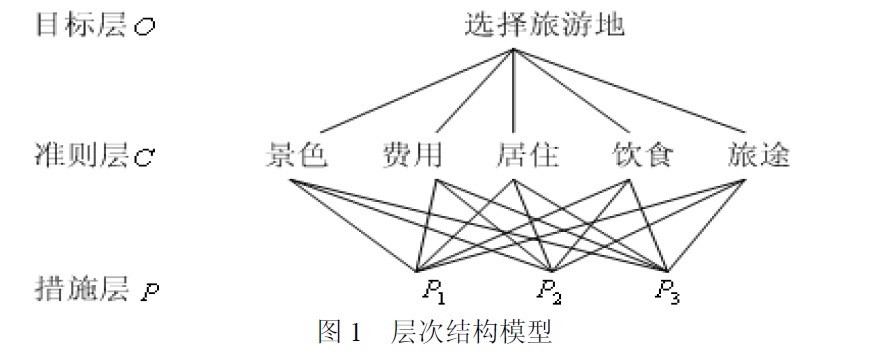
\includegraphics[scale=0.5]{Models/evaluation/AHP/Hierarchical model.png}
    \caption{Hierarchical model.}
    \label{fig:Hierarchical model}
\end{figure}

%%构造判断矩阵
(b)Construct the judgment matrix

(1)Construct the judgment matrix of $M-C$: Compare the elements of the criterion level in pairs to get the judgment matrix (see in Table \ref{tbl:Judgment matrix of O-C}).

\begin{table}[H]
    \renewcommand\arraystretch{2}   %%控制行间距
    \centering
    \begin{tabular}{llll}    %%三列均左对齐
        \toprule  %%表格横线加粗
        \specialrule{0em}{2pt}{2pt}    %%添加透明线控制行高
        $O$ & $C_1$ & $C_2$ & $C_3$ \\
        \specialrule{0em}{2pt}{2pt}    %%添加透明线控制行高
        \hline
        \specialrule{0em}{1pt}{1pt}    %%添加透明线控制行高
        $C_1$ & 1.0000 & 3.0000 & 4.0000 \\
        $C_2$ & 0.3333 & 1.0000 & 2.0000 \\
        $C_3$ & 0.2500 & 0.5000 & 1.0000 \\    
        \specialrule{0em}{1pt}{1pt}    %%添加透明线控制行高
        \bottomrule
    \end{tabular}
    \caption{Judgment matrix of $O-C$.}
    \label{tbl:Judgment matrix of O-C}
\end{table}

%%计算特征值，权重向量
%%代码见python
After that, it is easy to solve the eigenvalues of the matrix $M-C$ and the max eigenvalue is $\lambda_{max} = 3.0184$, thus getting the weight vector is $\omega_i = {(0.6250,0.2385,0.1365)}^T$.

Now we make the consistency check.

Since the consistency index $CI = \frac{\lambda_{max}-n}{n-1}$ and the consistency ratio $CR = \frac{CI}{RI}$, where $RI$ is only relative to the matrix size (see in Table \ref{tbl:The value of RI}).

By calculating, we get $CR = 0.0176<0.1$, which passes the consistency check.

%%The value of RI
\begin{table}[H]
    \renewcommand\arraystretch{2}   %%控制行间距
    \centering
    \begin{tabular}{ccccccccc}    %%三列均左对齐
        \toprule  %%表格横线加粗
        \specialrule{0em}{2pt}{2pt}    %%添加透明线控制行高
        matrix size & 2 & 3 & 4 & 5 & 6 & 7 & 8 & 9 \\
        \specialrule{0em}{2pt}{2pt}    %%添加透明线控制行高
        \hline
        \specialrule{0em}{1pt}{1pt}    %%添加透明线控制行高
        $RI$        & 0 & 0.58 & 0.90 & 1.12 & 1.24 & 1.32 & 1.41 & 1.45  \\
        \specialrule{0em}{1pt}{1pt}    %%添加透明线控制行高
        \bottomrule
    \end{tabular}
    \caption{The value of $RI$.}
    \label{tbl:The value of RI}
\end{table}

(2)Construct the judgment matrix of $C_1-P$, $C_2-P$ and $C_3-P$

Same as the formal part, we continue to construct the judgment matrix of $C_1-P$, $C_2-P$ and $C_3-P$ (see in Table \ref{tbl:Judgment matrix of C1-P}, \ref{tbl:Judgment matrix of C2-P} and \ref{tbl:Judgment matrix of C3-P})

\begin{table}[H]
    \renewcommand\arraystretch{2}   %%控制行间距
    \centering
    \begin{tabular}{llllll}    %%三列均左对齐
        \toprule  %%表格横线加粗
        \specialrule{0em}{2pt}{2pt}    %%添加透明线控制行高
        $C_1$ & $P_1$ & $P_2$ & $P_3$ & $P_4$ & $P_5$ \\
        \specialrule{0em}{2pt}{2pt}    %%添加透明线控制行高
        \hline
        \specialrule{0em}{1pt}{1pt}    %%添加透明线控制行高
        $P_1$ & 1.0000 & 3.0000 & 4.0000 & 1.0000 & 1.0000 \\
        $P_2$ & 0.3333 & 1.0000 & 2.0000 & 1.0000 & 1.0000 \\
        $P_3$ & 0.2500 & 0.5000 & 1.0000 & 1.0000 & 1.0000 \\
        $P_4$ & 1.0000 & 1.0000 & 1.0000 & 1.0000 & 1.0000 \\
        $P_5$ & 1.0000 & 1.0000 & 1.0000 & 1.0000 & 1.0000 \\
        \specialrule{0em}{1pt}{1pt}    %%添加透明线控制行高
        \bottomrule
    \end{tabular}
    \caption{Judgment matrix of $C_1-P$.}
    \label{tbl:Judgment matrix of C1-P}
\end{table}

\begin{table}[H]
    \renewcommand\arraystretch{2}   %%控制行间距
    \centering
    \begin{tabular}{lll}    %%三列均左对齐
        \toprule  %%表格横线加粗
        \specialrule{0em}{2pt}{2pt}    %%添加透明线控制行高
        $C_2$ & $P_6$ & $P_7$ \\
        \specialrule{0em}{2pt}{2pt}    %%添加透明线控制行高
        \hline
        \specialrule{0em}{1pt}{1pt}    %%添加透明线控制行高
        $P_6$ & 1.0000 & 3.0000 \\
        $P_7$ & 0.3333 & 1.0000 \\
        \specialrule{0em}{1pt}{1pt}    %%添加透明线控制行高
        \bottomrule
    \end{tabular}
    \caption{Judgment matrix of $C_2-P$.}
    \label{tbl:Judgment matrix of C2-P}
\end{table}

\begin{table}[H]
    \renewcommand\arraystretch{2}   %%控制行间距
    \centering
    \begin{tabular}{lll}    %%三列均左对齐
        \toprule  %%表格横线加粗
        \specialrule{0em}{2pt}{2pt}    %%添加透明线控制行高
        $C_3$ & $P_8$ & $P_9$ \\
        \specialrule{0em}{2pt}{2pt}    %%添加透明线控制行高
        \hline
        \specialrule{0em}{1pt}{1pt}    %%添加透明线控制行高
        $P_8$ & 1.0000 & 5.0000 \\
        $P_9$ & 0.2000 & 1.0000 \\
        \specialrule{0em}{1pt}{1pt}    %%添加透明线控制行高
        \bottomrule
    \end{tabular}
    \caption{Judgment matrix of $C_3-P$.}
    \label{tbl:Judgment matrix of C3-P}
\end{table}

By calculating, we get $CR_1 = 0.0785<0.1$, $CR_2 = 0.0000<0.1$, $CR_3 = 0.0000<0.1$, all of which pass the consistency check.

(c)model conclusion

From the formal four judgment matrices, we can calculate the total weights of each element in the plan level (see in table \ref{tbl:Element weights})

\begin{table}[H]
    \renewcommand\arraystretch{2}   %%控制行间距
    \centering
    \begin{tabular}{ll}    %%三列均左对齐
        \toprule  %%表格横线加粗
        \specialrule{0em}{2pt}{2pt}    %%添加透明线控制行高
        Evaluation index & Weight \\
        \specialrule{0em}{2pt}{2pt}    %%添加透明线控制行高
        \hline
        \specialrule{0em}{1pt}{1pt}    %%添加透明线控制行高
        $P_1$ & 0.1789 \\
        $P_2$ & 0.1594 \\
        $P_3$ & 0.1584 \\
        $P_4$ & 0.1535 \\
        $P_5$ & 0.1137 \\
        $P_6$ & 0.0906 \\
        $P_7$ & 0.0631 \\
        $P_8$ & 0.0596 \\
        $P_9$ & 0.0227 \\
        \specialrule{0em}{1pt}{1pt}    %%添加透明线控制行高
        \bottomrule
    \end{tabular}
    \caption{Element weights.}
    \label{tbl:Element weights}
\end{table}

Until now, we can set the whole index system of the evaluation of xxx (see in Figure \ref{fig:Index system}).

\begin{figure}[H]
    \centering
    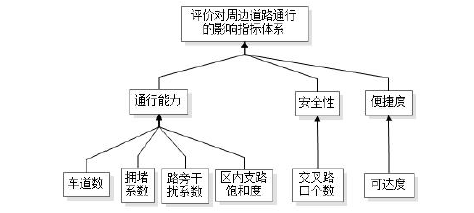
\includegraphics[scale=0.5]{Models/evaluation/AHP/Index system.png}
    \caption{Index system}
    \label{fig:Index system}
\end{figure}